\documentclass[a4paper, 10pt]{article}
\usepackage[T2A]{fontenc}
\usepackage[left=2cm,right=2cm,top=2cm,bottom=2cm]{geometry}
\usepackage[russian]{babel}
\usepackage{amsfonts,amsmath,amssymb}
\usepackage{mathrsfs}
\usepackage{graphicx}
\usepackage[normalem]{ulem}
\usepackage{wrapfig}
\usepackage{fancyhdr}
\usepackage{floatflt}
\usepackage{python}
\usepackage{float}
\usepackage{ amssymb }
\usepackage{indentfirst}
\usepackage{setspace}
\usepackage{scrextend}
\usepackage{listings}
\usepackage{makecell,tabularx}
\usepackage{hyperref}
\usepackage{xcolor}

\newcommand{\rub}{{\rm{Р}\kern-.635em\rule[.5ex]{.52em}{.04em}\kern.11em}}

\definecolor{linkcolor}{HTML}{000000} 
\definecolor{urlcolor}{HTML}{0000FF} 

\hypersetup{pdfstartview=FitH,  linkcolor=linkcolor,urlcolor=urlcolor, colorlinks=true}

\definecolor{grey}{RGB}{40, 40, 40}

\renewcommand{\href}[1]{\url{#1}}

\lstdefinestyle{CommentStyle}{
    language=XML,
    %numbers=left, numberstyle=\tiny, stepnumber=1, numbersep=5pt,
    commentstyle=\color{red},
	basicstyle=\footnotesize\ttfamily,
	language={[ANSI]C++},
	keywordstyle=\bfseries,
	showstringspaces=false,
	morekeywords={include, printf},
	commentstyle={},
	escapeinside=§§,
	escapebegin=\begin{russian}\commentfont,
	escapeend=\end{russian},
    keywordstyle=\color{blue}\bfseries,
    morekeywords={align,begin},
    extendedchars=\true,
    tabsize=2
}
\lstdefinestyle{myLatexStyle}{
    language=c++,
    %backgroundcolor=\color{grey},
    numbers=left, numberstyle=\tiny, stepnumber=1, numbersep=5pt,
    commentstyle=\color{red},
    keywordstyle=\color{blue}\bfseries,
    morekeywords={align,begin},
    extendedchars=\true,
    tabsize=2
}

\lstdefinestyle{pmyLatexStyle}{
    language=java,
    %backgroundcolor=\color{grey},
    numbers=left, numberstyle=\tiny, stepnumber=1, numbersep=5pt,
    commentstyle=\color{red},
    keywordstyle=\color{blue}\bfseries,
    morekeywords={align,begin},
    extendedchars=\true,
    tabsize=2
}

\setlength{\parindent}{12,5mm}

\newcommand{\bvec}[1]{\overrightarrow{#1}}
\newcommand{\mcol}[1]{\multicolumn{2}{c}{#1}}
\newcommand{\mcolt}[1]{&#1&}
\renewcommand{\a}{\vec{a}}
\renewcommand{\b}{\vec{b}}
\renewcommand{\c}{\vec{c}}
\renewcommand{\d}{\vec{d}}
\renewcommand{\i}{\vec{i}}
\renewcommand{\j}{\vec{j}}
\renewcommand{\k}{\vec{k}}
\newcommand{\nul}{\vec{0}}

\newcommand{\logo}{\vcenter{\hbox{\includegraphics[width=.8em]{/Users/pluttan/Documents/bw2.png}}}}
\onehalfspacing

\pagestyle{fancy}
\renewcommand{\sectionmark}[1]{\markright{#1}}
\fancyhf{} 
\fancyhead[R]{\bfseries\thepage}
\fancyhead[LO]{$\mathfrak{Copyright}\ \mathfrak{pluttan} \logo$}

\newcommand{\image}[2]{
	\begin{figure}[H]
		\center{\includegraphics[height=#2pt]{img/#1} }
    \end{figure}
}

\newcommand{\dotitle}[3]{

\thispagestyle{empty}
\sloppy{
  \scriptsize{
    \line(6,0){0}

    \centering $\mathfrak{Copyright}\ \mathfrak{pluttan} \logo$

    \centering Привет! Меня зовут Андрей, я создаю свою ботву, этот файл малая ее часть. 
    
    \centering Пользоваться и распространять файлы конечно же можно. Если вы нашли ошибку в файле, можете 
    
    \centering исправить ее в исходном коде и подать на слияние или просто написать в issue. 
    
    \centering Приятного бота)

    \line(6,0){300}

    \centering GitHub: https://github.com/pluttan

    \line(6,0){0}
  }}

\topskip=-200pt
\vspace*{130pt}
\begin{Huge}
  \textbf{
    \begin{center}
        #1
    \end{center}
  }
  {\begin{center} 
        #2
    \end{center}}
\end{Huge}
\vspace*{300pt}
  \begin{flushright}
    Над файлом работали: \\
    pluttan\\
    #3
  \end{flushright}
\newpage
\pagestyle{fancy}
\renewcommand{\sectionmark}[1]{\markright{#1}}
\fancyhf{} 
\fancyhead[R]{\bfseries\thepage}
\fancyhead[LO]{$\mathfrak{Copyright}\ \mathfrak{pluttan} \logo$}
}


% It's XeLaTeX, if you can't compile comment this line 
\usepackage{fontspec}\setmainfont{Times New Roman} 

\include{/Users/pluttan/Documents/forMyDocs/preambMisha.tex}
\newcommand{\df}[2]{\noindent
% $\blacktriangleright$
 \textbf{#1} - #2
% $\blacktriangleleft$
}
\newcommand{\dfn}[2]{\noindent
% $\blacktriangleright$ 
\textbf{#1} #2
% $\blacktriangleleft$
}
\newcommand{\dft}[3]{\noindent
% $\blacktriangleright$ 
#1 \textbf{#2} #3
% $\blacktriangleleft$
}
\newcommand{\ep}{\begin{FlushRight} ЧТД\end{FlushRight}}

\begin{document}
\tikz[remember picture,overlay] \node[opacity=0.1,inner sep=0pt] at (current page.center){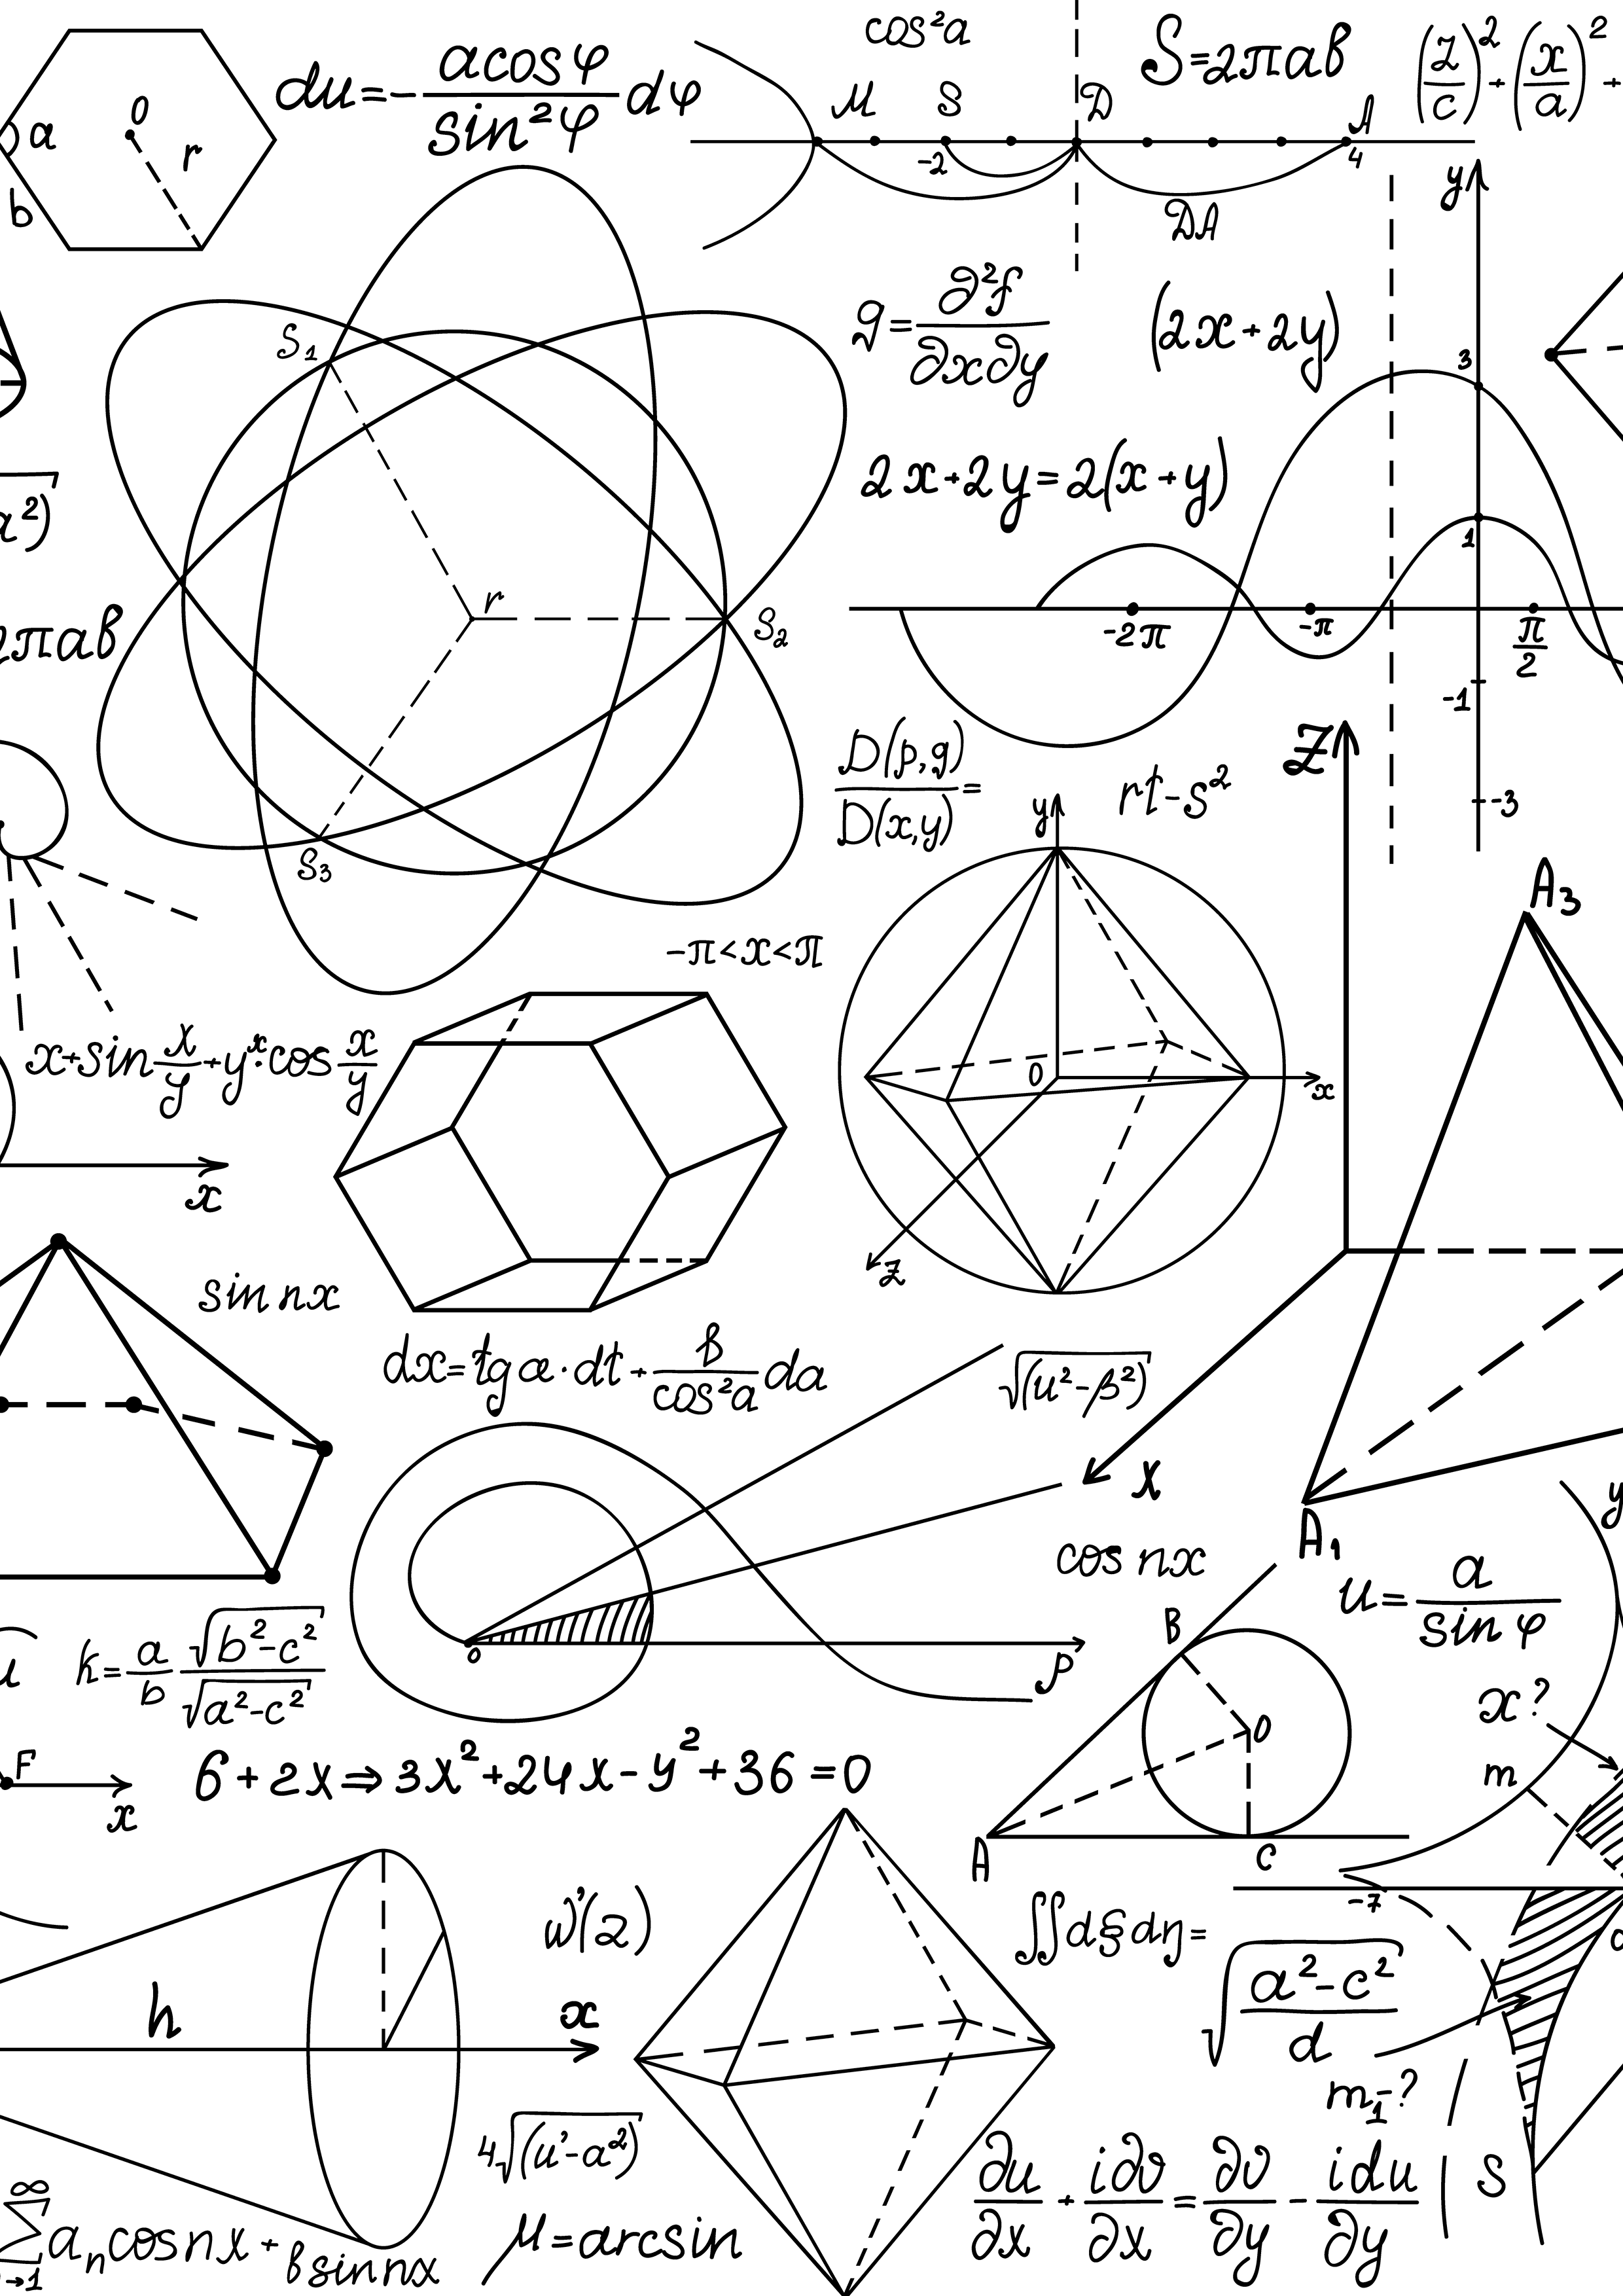
\includegraphics[width=\paperwidth,height=\paperheight]{../img/bg.png}};
\dotitle{Подготовка к РК2}{Аналитическая геометрия}
\large
\section{Базовые теоретические вопросы}

\subsection{Дать определение единичной, нулевой, верхней треугольной и нижней треугольной матрицы.}

\df{Единичная матрица}{квадратная матрица, для элементов которой выполняется следующее условие: $a_{ij} = \begin{cases}0, i \ne j\\ 1, i = j\end{cases}$}

т.е. элементы главной диагонали равны 1, остальные 0.

Обозначение $[E]$

\vspace*{15pt}

\df{Нулевая матрица}{матрица, все элементы которой равны 0, т.е. $a_{ij} = 0, \forall i, j$}

Обозначение $[\Theta]$

\vspace*{15pt}

\df{Верхняя треугольная матрица}{квадратная матрица, все элементы под главной диагональю которой равны 0.}

\vspace*{15pt}

\df{Нижняя треугольная матрица}{квадратная матрица, все элементы над главной диагональю которой равны 0.}

\subsection{Дать определение равенства матриц.}

Матрицы называются {\bf{равными}}, если:
\begin{enumerate}
    \item[1)] они имеют одинаковый тип,
    \item[2)] У них совпадают все соответствующие элементы.
\end{enumerate}

 \begin{center} 
    Для $A = (a_{ij})$ и $B = (b_{ij})$
 
    $A = B \iff A, B \in M_{mn}(\mathbb{R})$ и $a_{ij} = b_{ij}$ $\forall ij$  
\end{center}



\subsection{Дать определение суммы матриц и произведения матрицы на число.}

\df{Сумма матриц $A = (a_{ij})$ и $B = (b_{ij})$ одного типа $m\times n$}{матрица $C = (c_{ij})$ того же типа $m\times n$ с элементами $c_{ij} = a_{ij} + b_{ij}$.}

\vspace*{15pt}

\df{Произведение матрицы $A = (a_{ij})$ типа $m\times n$ на число $\alpha \in \mathbb{R}$}{матрица $C = (c_{ij})$ того же типа $m\times n$ с элементами $c_{ij} = \alpha a_{ij}$.}

\subsection{Дать определение операции транспонирования матриц.}

\dft{Для матрицы $A = (a_{ij})$ типа $m\times n$ }{ее транспонированной матрицей}{называется матрица $A^T = (c_{ij})$ типа $n\times m$ с элементами $c_{ij} = a_{ji}$}

При транспонировании матрицы ее строки (столбцы) страновятся столбцами (строками) с теми же номерами.

\subsection{Дать определение операции умножения матриц.}

\dfn{Произведением матрицы $A = (a_{ij})$ типа $m\times n$ и матрицы $B = (b_{ij})$ типа $n\times p$}{называется матрица $C = (c_{ij})$ типа $m \times p$ с элементами $c_{ij} = \overset{n}{\underset{k = 1}{\sum}}a_{ik}b_{kj} = a_{i1}b_{1j}+...+a_{in}b_{nj}$.}

$$
\begin{pmatrix} 
    a_{11}&a_{12}&\ldots&a_{1n}\\ 
    \vdots&\vdots&\ddots&\vdots\\
    \mathbf{a_{i1}}&\mathbf{a_{i2}}&\mathbf{\ldots}&\mathbf{a_{in}}\\ 
    \vdots&\vdots&\ddots&\vdots\\
    a_{m1}&a_{m2}&\ldots&a_{mn}\\ 
\end{pmatrix}
\times
\begin{pmatrix} 
    b_{11}&\ldots&\mathbf{b_{1j}}&\ldots&b_{1p}\\ 
    b_{21}&\ldots&\mathbf{b_{2j}}&\ldots&b_{2p}\\ 
    \vdots&\ddots&\mathbf{\vdots}&\ddots&\vdots\\
    b_{n1}&\ldots&\mathbf{b_{nj}}&\ldots&b_{np}\\ 
\end{pmatrix}
=
\begin{pmatrix} 
    c_{11}&c_{12}&\ldots&c_{1j}&\ldots&c_{1p}\\ 
    c_{21}&c_{22}&\ldots&c_{2j}&\ldots&c_{2p}\\ 
    \vdots&\vdots&\ddots&\vdots&\ddots&\vdots\\
    c_{i1}&c_{i2}&\ldots&\mathbf{c_{ij}}&\ldots&c_{ip}\\ 
    \vdots&\vdots&\ddots&\vdots&\ddots&\vdots\\
    c_{m1}&c_{m2}&\ldots&c_{mj}&\ldots&c_{mp}\\ 
\end{pmatrix}
$$

$AB \ne BA$ (как правило).

\subsection{Дать определение обратной матрицы.}

\dft{Пусть $A$ - квадратная матрица порядка $n$. Матрица $B$ называется}{обратной}{к матрице $A$, если:
\begin{enumerate}
    \item Она того же порядка $n$,
    \item $AB = BA = E$, где $E$ - единичная матрица.
\end{enumerate}
}

\subsection{Дать определение минора. Какие миноры называются окаймляющими для данного минора матрицы?}

{\bf{Минором}} порядка $k$ матрицы $A$ типа $m\times n$ называется определитель, который составлен из элементов этой матрицы, стоящих на пересечении любых $k$ строк и $k$ столбцов с сохранением порядка этих строк и столбцов.

Обозначение: минор $M^{j_1 ... j_k}_{i_1 ... i_k}$ составлен из элементов, расположенных на пересечении строк $i_1, ..., i_k$ и столбцов $j_1, ..., j_k$, причем $i_1<...<i_k$, $j_1<...<j_k$.

\vspace*{15pt}

Минор $M'$ матрицы $A$ называется {\bf{окаймляющим}} для минора $M$, если он получается из $M$ добавлением одной новой строки и одного нового столбца, причем эти строка и столбец входят в матрицу $A$ и не входят в минор $M$.

\subsection{Дать определение базисного минора и ранга матрицы.}

\df{Ранг матрицы}{число, равное максимальному проядку среди ее ненулевых миноров.}

\vspace*{15pt}

\dft{Минор $M$ матрицы $A$ называется}{базисным,}{если
\begin{enumerate}
    \item[1)] он не равен нулю,
    \item[2)] его порядок равен $RgA$.
\end{enumerate}
}

У матрицы может быть несколько базисных миноров.

\subsection{Дать определение однородной и неоднородной СЛАУ.}

\dfn{Системой линейных алгебраических уравнений}{называется система вида 
$$
\begin{cases}
    a_{11}x_1+a_{12}x_2+\ldots+a_{1n}x_n = b_1\\
    a_{21}x_1+a_{22}x_2+\ldots+a_{2n}x_n = b_2\\
    \ldots\ldots\ldots\ldots\ldots\ldots\ldots\ldots\ldots\ldots\ldots\\
    a_{m1}x_1+a_{m2}x_2+\ldots+a_{mn}x_n = b_m
\end{cases}
$$
Где $a_{ij}, b_i, x_i \in \mathbb{R}$
}

Числа $a_{ij}$ называются коэффициентами системы,
$b_{ij}$ называется свободными членами.

СЛАУ называется {\bf{однородной}}, если все $b$ равны $0$, {\bf{неоднородной}}, если хотя бы один из $b_i$ не равен $0$.

\subsection{Дать определение фундаментальной системы решений однородной СЛАУ.}

Пусть дана однородная СЛАУ $AX = \Theta$ с $n$ неизвесными $x_1, ..., x_n$, и пусть $RgA = r$. Фундаментальной системой решений (ФСР) однородной СЛАУ $AX = \Theta$ называется любой набор из $k = n - r$ линейно независимых столбцов $x^{(1)}, ..., x^{(k)}$ является решениями этой системы.

\subsection{Записать формулы для нахождения обратной матрицы к произведению двух обратимых матриц и для транспонированной матрицы.}

Обратная матрица к произведению двух обратимых матриц: если квадратные матрицы $A$ и $B$ одного порядка и имеют обратные матрицы $A^{-1}$ и $B^{-1}$, то их произведение $AB$ имеет обратную матрицу $AB^{-1}$, причем $(AB)^{-1} = B^{-1}A^{-1}$.

\vspace*{15pt}

Обратная матрица для транспонированной матрицы: если квадратная матрица $A$ имеет обратную матрицу $A^{-1}$, то транспонированная матрица $A^T$ тоже имеет обратную матрицу $(A^T)^{-1}$, причем $(A^T)^{-1} = (A^{-1})^T$.

\subsection{Дать определение присоединённой матрицы и записать формулу для вычисления обратной матрицы.}

{\bf{Присоединеной матрицей}} для квадратной матрицы $A$ называется матрица $A^* = (A_{ji})$, где $(A_{ij})$ - матрица из алгебраических дополнений для соответствующих элементов.

Формула для вычисления обратной матрицы
$$A^{-1} = \frac{1}{detA}A^*$$

%note : искуственный переход на новую страницу
\vspace*{15pt}
\vspace*{15pt}

\subsection{Перечислить элементарные преобразования матриц.}

Элементарные преобразования матриц
\begin{enumerate}
    \item[1)] Умножение строки (столбца) матрицы на число $\lambda \ne 0$:
    \item[2)] Перестановка двух строк (столбцов).
    \item[2)] Добавление к одной строке (столбцу) матрицы другой строки (столбца), умноженной на число.
\end{enumerate}

\subsection{Записать формулы Крамера для решения системы линейных уравнений с обратимой матрицей.}

СЛАУ $AX = B$, где $A$ - квадратная и $detA \ne 0$, имеет единственное решение, причем $x_1 = \frac{\Delta_1}{\Delta}, ..., x_n = \frac{\Delta_n}{\Delta}$, где $\Delta = detA$,
$$\Delta_1 = 
\begin{vmatrix}
    b_1&a_{12}&\ldots&a_{1n}\\
    \vdots&\vdots&\ddots&\vdots\\
    b_n&a_{n2}&\ldots&a_{nn}\\
\end{vmatrix}, ..., 
\Delta_n = 
\begin{vmatrix}
    a_{11}&\ldots&a_{1n-1}&b_1\\
    \vdots&\ddots&\vdots&\vdots\\
    a_{n1}&\ldots&a_{nn-1}&b_n\\
\end{vmatrix}
$$

\subsection{Перечислить различные формы записи системы линейных алгебраических уравнений (СЛАУ). Какая СЛАУ называется совместной?}

\noindent
Формы записи СЛАУ:
\begin{enumerate}
    \item Координатная: 
    $$
    \begin{cases}
        a_{11}x_1+a_{12}x_2+\ldots+a_{1n}x_n = b_1\\
        a_{21}x_1+a_{22}x_2+\ldots+a_{2n}x_n = b_2\\
        \ldots\ldots\ldots\ldots\ldots\ldots\ldots\ldots\ldots\ldots\ldots\\
        a_{m1}x_1+a_{m2}x_2+\ldots+a_{mn}x_n = b_m
    \end{cases}
    a_{ij}, b_i, x_i \in \mathbb{R}
    $$
    \item Векторная:
    $$x_1
    \begin{pmatrix}
        a_{11}\\a_{21}\\\ldots\\a_{m1}
    \end{pmatrix}+x_2
    \begin{pmatrix}
        a_{12}\\a_{22}\\\ldots\\a_{m2}
    \end{pmatrix}+...+x_n
    \begin{pmatrix}
        a_{1n}\\a_{2n}\\\ldots\\a_{mn}
    \end{pmatrix}=
    \begin{pmatrix}
        b_{1}\\b_{2}\\\ldots\\b_{m}
    \end{pmatrix}
    $$
    \begin{center} или \end{center}
    $$
    x_1\vec{a_1}+x_2\vec{a_2}+...+x_n\vec{a_n} = \vec{b}
    $$
    \item Матричная:
    $$
    \begin{pmatrix}
        a_{11}&a_{12}&\ldots&a_{1n}\\
        a_{21}&a_{22}&\ldots&a_{2n}\\
        \vdots&\vdots&\ddots&\vdots\\
        a_{m1}&a_{m2}&\ldots&a_{mn}
    \end{pmatrix}
    \begin{pmatrix}
        x_{1}\\x_{2}\\\vdots\\x_{m}
    \end{pmatrix} = 
    \begin{pmatrix}
        b_{1}\\b_{2}\\\vdots\\b_{m}
    \end{pmatrix}
    $$
    \begin{center} или \end{center}
    $$
    AX = B \text{ } (A\vec{x} = \vec{b})
    $$
    
\end{enumerate}

СЛАУ называется совместной (несовместной), если она имеет (не имеет) решение.

\subsection{Привести пример, показывающий, что умножение матриц некоммутативно.}

Некомутативность произведение матриц: $AB\ne BA$ (как правило, но бывают исключения)

$A = \begin{pmatrix}1&0\\0&0\end{pmatrix}, 
           B = \begin{pmatrix}0&1\\0&0\end{pmatrix}$ :  $
           AB = \begin{pmatrix}0&1\\0&0\end{pmatrix},
           BA = \begin{pmatrix}0&0\\0&0\end{pmatrix}
           \Rightarrow AB \ne BA$
\vspace*{15pt}

$A = \begin{pmatrix}1&2\end{pmatrix}, 
           B = \begin{pmatrix}3\\4\end{pmatrix}$ :  $
           AB = \begin{pmatrix}11\end{pmatrix},
           BA = \begin{pmatrix}3&6\\4&8\end{pmatrix}
           \Rightarrow AB \ne BA$


\subsection{Сформулировать свойства ассоциативности умножения матриц и дистрибутивности умножения относительно сложения.}

\noindent
Свойства умножения матриц:
\begin{enumerate}
    \item[1)] Ассоциативность $(AB)C = A(BC)$.
    \item[2)] Дистрибутивность $(A + B)C = AC + BC$.
\end{enumerate}

\subsection{Сформулировать критерий Кронекера — Капелли совместности СЛАУ.}

Система $AX = B$ совместна $\iff$ ранг расширенной матрицы равен рангу матрицы, т.е. $Rg(A|B)=RgA$

\subsection{Сформулировать теорему о базисном миноре.}

Теорема о базисном миноре:
\begin{enumerate}
    \item Базисные строки (столбцы) матрицы $A$, соответствующие любому базисному минору $M$, линейно независимы.
    \item Любые строки (столбцы) матрицы $A$, не входящие в базисный минор $M$, являются линейными комбинациями базисных строк (столбцов).
\end{enumerate}

\subsection{Сформулировать теорему о свойствах решений однородной СЛАУ.}

Если $X^{(1)}, ..., X^{(S)}$ - решения однородной СЛАУ, то любая их линейная комбинация $X = \alpha_1X^{(1)}+ ...+ \alpha_sX^{(S)}, \alpha_i\in\mathbb{R}$, тоже является решением.

\subsection{Сформулировать теорему о структуре общего решения неоднородной СЛАУ.}

Пусть $X^0$ - некоторое решение неоднородной СЛАУ $AX = B$, 

$X^{(1)}, ..., X^{(k)}$ - ФСР соответствующей однородной СЛАУ $AX = \Theta.$

Тогда любое решение $X$ неоднородной СЛАУ $AX = B$ можно представить в виде:
$$X = X^0 + c_1X^{(1)}+ ...+ c_kX^{(k)},$$
где $c_i\in\mathbb{R}, i = 1, ..., k$.

\subsection{Сформулировать теорему о структуре общего решения однородной СЛАУ.}

Пусть $X^{(1)}, ..., X^{(k)}$ - любая ФСР однородной СЛАУ $AX = \Theta.$

Тогда любое решение $X$ этой системы можно представить как линейную комбинацию ФСР:$$X = c_1X^{(1)}+ ...+ c_kX^{(k)}, \text{ где } c_i\in\mathbb{R}$$

\subsection{Сформулировать теорему об инвариантности ранга при элементарных преобразованиях матрицы.}

При элементарных преобразованиях матрицы ее ранг не меняется.

\subsection{Сформулировать критерий существования обратной матрицы.}

Для квадратной матрицы $A$ $\exists$ обратная матрица $A^{-1} \iff detA \ne 0$
(т.е. когда $A$ - невырожденная матрица). 

\newpage\section{Теоретические вопросы повышенной сложности}

\subsection{Доказать теорему о связи решений неоднородной и соответствующей однородной СЛАУ и теорему о структуре общего решения неоднородной СЛАУ.}

\textit {Теорема (о связи решений неоднородной и соответствующей однородной СЛАУ).}

\vspace*{15pt}

Пусть $X^0$ - некоторое решение неоднородной СЛАУ $AX = B$, тогда:

$X$ - решение этой же СЛАУ $\iff X = X^0 + Y$, где $Y$ - некоторое решение соответствующей однородной СЛАУ $AX = \Theta$.

\vspace*{15pt}

{\bf {Доказательство}}

($\Rightarrow$)  

Пусть $X^0$, $X$ - решения неоднородной СЛАУ $AX = B$. Рассмотрим $Y = X - X^0$ и найдем $AY$:

$AY = A(X - X^0) = AX - AX^0 = B - B = \Theta$, т.е. $AY = \Theta$, а значит, $Y$ - решение однородной СЛАУ $AX = \Theta$ и $X = X^0 + Y$.

\vspace*{15pt}

($\Leftarrow$)  

Пусть $X^0$ - решение неоднородной СЛАУ $AX = B$ (т.е. $AX^0 = B$),

а $Y$ - решение однородной СЛАУ $AX = \Theta$ (т.е. $AY = \Theta$).

Рассмотрим $X = X^0 + Y$ и найдем AX:

$AX = A(X^0 + Y) = AX^0 + AY = B + \Theta = B$, т.е. $X$ - решение неоднородной СЛАУ $AX = B$.  

\ep


\textit {Теорема (о структуре общего решения неоднородной СЛАУ).} 

\vspace*{15pt}

Пусть $X^0$ - некоторое решение неоднородной СЛАУ $AX = B$,

$X^{(1)}, ..., X^{(k)}$ - ФСР (фундаментальная система решений) соответствующей однородной СЛАУ $AX = \Theta$.

Тогда любое решение $X$ неоднородной СЛАУ $AX = B$ можно представить в виде:
$$X = X^0 + c_1X^{(1)} + ... + c_kX^{(k)}, \text{ где } c_i \in \mathbb{R}, i = 1, ..., k.$$

{\bf {Доказательство}}

Пусть $X^0$ - некоторое решение неоднородной СЛАУ $AX = B$, $X$ - любое решение той же системы.

Тогда по теореме о связи решений неоднородной и соответствующей однородной СЛАУ:
$X = X^0 + Y$, где $Y$ - некоторое решение соответствующей однородной СЛАУ.

По теореме о структуре общего решения однородной СЛАУ:

$Y = c_1X^{(1)} + ... +  c_kX^{(k)}$, где $X^{(1)}, ..., X^{(k)}$ - ФСР однородной СЛАУ, $c_i \in \mathbb{R}$. Следовательно $X = X^0 + c_1X^{(1)} + ... + c_kX^{(k)}$.  

\ep

\subsection{Доказать свойства ассоциативности и дистрибутивности умножения матриц. }

\textit {Свойство ассоциативности умножения матриц: $(AB)C = A(BC)$}

\vspace*{15pt}

{\bf {Доказательство}}

\vspace*{15pt}

$\overbrace{\underbrace{(AB)}_{D}C}^{X} = \overbrace{A\underbrace{(BC)}_{F}}^{Y}$


Докажем, что матрицы $X$ и $Y$:
\begin{enumerate}
    \item[1)] имеют одинаковый тип,
    \item[2)] их соответствующие элементы равны: $x_{ij} = y_{ij}$ 
\end{enumerate}

    $
    \begin{array}{ c|c } 
     \text {матрицы} & \text{типа} \\
     \hline
     A = (a_{ij}) & m \times n \\ 
     B = (b_{ij}) & n \times k \\ 
     D = (d_{ij}) & m \times k \\  
     C = (c_{ij}) & k \times l \\ 
     F = (f_{ij}) & n \times l \\ 
     X = (x_{ij}) & \mathbf{m \times l} \\ 
     Y = (y_{ij}) & \mathbf{m \times l} \\ 
    \end{array}
    % TODO : вертикальная фигурна скобка на две последние строчки с текстом (см фото в вк)
    $

    \vspace*{15pt}
    $x_{ij} =\overset{k}{\underset{r = 1}{\sum}}d_{ir}c_{rj} = \overset{k}{\underset{r = 1}{\sum}}(\overset{n}{\underset{s = 1}{\sum}}a_{is}b_{sr})c_{rj} = \overset{k}{\underset{r = 1}{\sum}}(\overset{n}{\underset{s = 1}{\sum}}a_{is}b_{sr}c_{rj})$,
    
    $y_{ij} = \overset{n}{\underset{s = 1}{\sum}}a_{is}f_{sj} = \overset{n}{\underset{s = 1}{\sum}}(a_{is}(\overset{k}{\underset{r = 1}{\sum}}b_{sr}c_{rj})) = \overset{n}{\underset{s = 1}{\sum}}(\overset{k}{\underset{r = 1}{\sum}}a_{is}b_{sr}c_{rj}) = \overset{k}{\underset{r = 1}{\sum}}(\overset{n}{\underset{s = 1}{\sum}}a_{is}b_{sr}c_{rj})$, т.е. $x_{ij} = y_{ij}$.

    \ep

    \textit {Свойство дистрибутивности умножения матриц: $(A + B)C = AC + BC$}

    \vspace*{15pt}

    {\bf{Доказательство}}
    
    \vspace*{15pt}

    $\overbrace{\underbrace{(A + B)}_{X}C}^{Y} = \underbrace{(AC)}_{Z} +\underbrace{(BC)} _{W}$

    Докажем, что матрицы $Y$ и $Z + W$:
\begin{enumerate}
    \item[1)] имеют одинаковый тип,
    \item[2)] их соответствующие элементы равны: $y_{ij} = z_{ij} + w_{ij}$ 
\end{enumerate}

$
    \begin{array}{ c|c } 
     \text {матрицы} & \text{типа} \\
     \hline
     A = (a_{ij}) & m \times n \\ 
     B = (b_{ij}) & m \times n \\ 
     X = (x_{ij}) & m \times n \\  
     C = (c_{ij}) & n \times k \\ 
     Y = (y_{ij}) & \mathbf{m \times k} \\ 
     Z = (z_{ij}) & \mathbf{m \times k} \\ 
     W = (w_{ij}) & \mathbf{m \times k} \\ 
    \end{array} 
$

    \vspace*{15pt}
    $y_{ij} = \overset{n}{\underset{r = 1}{\sum}}x_{ir}c_{rj} = \overset{n}{\underset{r = 1}{\sum}}(a_{ir} + b_{ir})c_{rj} = \overset{n}{\underset{r = 1}{\sum}}(a_{ir}c_{rj} + b_{ir}c_{rj}) = \overset{n}{\underset{r = 1}{\sum}}a_{ir}c_{rj} + \overset{n}{\underset{r = 1}{\sum}}b_{ir}c_{rj} = z_{ij} + w_{ij}$.  

    \ep

\subsection{Доказать теорему о базисном миноре.}
\textit {Теорема о базисном миноре}
\begin{enumerate}
    \item Базисные строки (столбцы) матрицы $A$, соответствующие любому базисному минору $M$, линейно независимы.
    \item Любые строки (столбцы) матрицы $A$, не входящие в базисный минор $M$, являются линейными комбинациями базисных строк (столбцов).
\end{enumerate}

\vspace*{15pt}

{\bf{Доказательство (для строк)}}

\vspace*{15pt}

Пусть матрица $A = (a_{ij})$ имеет тип $m \times n$, пусть $RgA = r$ и пусть $M$ - базисный минор матрицы $A$.

Рассмотрим строки, на которых построен $M$. Это базисные строки матрциы $A$.

\begin{enumerate}
    \item Докажем, что базисные строки линейно независимы.
    
    Пусть от противного они линейно зависимы $\overset{\text{по критерию}}{\Rightarrow}$ хотя бы одна строка из них в матрице $A$ является линейной комбинацией остальных $\Rightarrow$ в миноре $M$ хотя бы одна строка является линейной комбинацией остальных $\overset{\text{по св-ву det}}{\Rightarrow}$ $detM = 0$,
    
    Противоречие, т.к. $M$ - базисный минор.

    \item Докажем, что любая строка матрицы $A$, не входящая в базисный минор $M$, является линейной комбинацией базисных строк.

    Пусть базисный минор $M$ расположен в верхнем левом углу матрицы $A$:
    
    %матрица - минор
    %     |a(11) ... a(1r)|
    % M = |...       ...  |
    %     |a(r1) ... a(rr)|
    $$
    M = 
    \begin{pmatrix}
        a_{11}&\ldots&a_{1r}\\
        \vdots&\ddots&\vdots\\
        a_{r1}&\ldots&a_{rr}\\
    \end{pmatrix}
    $$
    Добавим к $M$ любую $i$-ю {\bf {не базисную}} строку и любой $j$-й столбец (возможно даже базисный):
    
    $$
    \Delta_j = 
    \begin{pmatrix}
        a_{11}&\ldots&a_{1r}&a_{1j}\\
        \vdots&&\vdots&\vdots\\
        a_{r1}&\ldots&a_{rr}&a_{rj}\\
        a_{i1}&\ldots&a_{ir}&a_{ij}\\
    \end{pmatrix}
    $$
Порядок $\Delta_j$ равен $r + 1$, следовательно $\Delta_j = 0.$

Разложим $\Delta_j$ по последнему столбцу:

$\Delta_j = a_{1j}A_{1j} + ... + a_{rj}A_{rj} + a_{ij}A_{ij} = 0$, где $A_{kj}$ - это алгебраические дополнения элементов $a_{kj}$ в $\Delta_j$.

Заметим, что
\begin{enumerate}
    \item[1)] эти алгебраические дополнения $A_{kj}$ не зависят от номера $j$, т.к. при их вычислении $j$-й столбец вычеркивается.
    \item[2)] $A_{ij} = (-1)^{(r + 1) + (r + 1)}M = (-1)^{2(r + 1)}M = M \ne 0,$
\end{enumerate}

Выразим элемент $a_{ij}:$

$$a_{ij} = \underbrace{\frac{-A_{1j}}{M}}_{b_1}a_{1j} - ... - \underbrace{\frac{-A_{rj}}{M}}_{b_r}a_{rj}, \text{ т.е.}$$ 

$$a_{ij} = b_1a_{1j} + ... + b_ra_{rj}, \text{ где } b_1, ..., b_r \text{ не зависят от номера j.}$$ 

Если поставить на место $j$-го столбца в $\Delta_j$ его $1$-й столбец, то получим

$$
\Delta_1 = 
\begin{pmatrix}
    a_{11}&\ldots&a_{1r}&a_{11}\\
    \vdots&&\vdots&\vdots\\
    a_{r1}&\ldots&a_{rr}&a_{r1}\\
    a_{i1}&\ldots&a_{ir}&a_{i1}\\
\end{pmatrix}
$$
и $\Delta_1 = a_{11}A_{1j} + ... + a_{r1}A_{rj} + a_{i1}A_{ij},$

выразим элемент $a_{i1}:$

$$a_{i1} = \underbrace{\frac{-A_{1j}}{M}}_{b_1}a_{11} - ... - \underbrace{\frac{-A_{rj}}{M}}_{b_r}a_{r1},\text{ т.е.}$$ 

$a_{i1} = b_1a_{11} + ... + b_ra_{r1}, $ (с теми же коэффициентами $b_1, ..., b_r$).

Аналогично ставим на место $j$-го столбца в $\Delta$ остальные столбцы по очереди и будем получать аналогичные равенства, в частности,
$$a_{ir} = b_1a_{1r} + ... + b_ra_{rr}.$$

Следовательно, вся $i$-я строка матрицы $A$ является линейной комбинацией ее первых $r$ строк (базисных) с коэффициентами $b_1, ..., b_k$.

\end{enumerate}

\ep

\subsection{Доказать критерий существования обратной матрицы.}

\textit{критерий существования обратной матрицы}

\vspace*{15pt}

Для квадратной матрицы $A$ $\exists$ обратная матрица $A^{-1}$ $\iff$ $detA \ne 0$ (т.е. когда $A$ - невырожденная матрица).

\vspace*{15pt}

{\bf {Доказательство}}

($\Rightarrow$)  

Пусть $\exists A^{-1}$. Докажем, что $detA \ne 0$.

По определению обратной матрицы, 
$$AA^{-1} = E.$$

Возьмем $det$ от левой и правой части:
$$det(AA^{-1}) = detE$$

По свойствам $det$:
$$detA\cdot detA^{-1} = 1,$$

произведение чисел равно 1 $\rightarrow$ $detA \ne 0$, $det(A^{-1}) \ne 0$.

\vspace*{15pt}

($\Leftarrow$)

Пусть $detA \ne 0$.

\begin{enumerate}
    \item Построим матрицу $A^{-1}:$
    \begin{enumerate}
        \item[1)] Найдем $\forall$ алгебраические дополнения $A_{ij}$ и составим из них матрицу $(A_{ij})$.
        \item[2)] Транспонируем матрицу $(A_{ij}):$
    $$(A_{ji}) = (A_{ij})^T$$
        \item[3)] Рассмотрим матрицу $B = (b_{ij})$, где $b_{ij} = \frac{A_{ji}}{detA}$, т.е. $B = \frac{1}{detA}(A_{ji})$
    \end{enumerate}
    \item Проверим, что построенная матрица $B$ и будет $A^{-1}$.

    В самом деле, $B$ - квадратная и осталось проверить, что $AB = E$ (и $BA = E$).

    Обозначим $AB$ через $C = (c_{ik})$

    Найдем $c_{ik} = \overset{n}{\underset{j = 1}{\sum}}a_{ij}b_{jk} = \overset{n}{\underset{j = 1}{\sum}}a_{ij}\frac{A_{kj}}{detA} = \frac{1}{detA}\overset{n}{\underset{j = 1}{\sum}}a_{ij}A_{kj} = \begin{cases}1, i = k\\ 0, i \ne k\end{cases}$ 
    
    т.к. ${\underset{j = 1}{\sum}}a_{ij}A_{kj} = \begin{cases}detA, i = k\\ 0, i \ne k \text{ (по т. о "фальшивом"\ разложении определителя*)}\end{cases}$

    Следовательно, $C = E$, и $AB = E$.
    Аналогично показывается, что $BA = E$.
    Из $1, 2 \Rightarrow$ $B$ является $A^{-1}$ для $A$.

\end{enumerate}

\ep

\subsection{Доказать критерий Кронекера — Капелли совместности СЛАУ.}
\textit{Критерий Кронекера — Капелли совместности СЛАУ}

\vspace*{15pt}

Система $AX = B$ совместна $\iff$ ранг расширенной матрицы = рангу матрицы, т.е. $Rg(A|B) = RgA$

\vspace*{15pt}

{\bf{Доказательство}}

($\Rightarrow$)  

Пусть система $AX = B$ совместна.
Докажем, что $Rg(A|B) = RgA$.
\begin{enumerate}
    \item [1)] Столбцы матрицы $A$ являются столбцами матрицы $(A|B)$ $\Rightarrow$ $RgA \leqslant Rg(A|B)$
    \item [2)] Докажем, что $RgA \geqslant Rg(A|B)$
\end{enumerate} 


Т.к. система $AX = B$ совместна, то $\exists$ ее решение $x_1, ..., x_n:$

$x_1 \vec{a_1} + ... + x_n \vec{a_n} = \vec{b}$

Пусть $\vec{a_1},...\vec{a_k}$ - базисные столбцы в матрице $A \Rightarrow$ по теореме о базисном миноре, столбцы $\vec{a_{k+1}}, ..., \vec{a_n}$ выражаются через столбцы $\vec{a_1},...\vec{a_k} \Rightarrow$ столбец $\vec{b}$ выражается через $\vec{a_1},... , \vec{a_k} \Rightarrow$ $\vec{a_1},... , \vec{a_k}$ - базисные столбцы в матрице $(A|B)$.

Это означает, что число базисных столбцов в матрице $(A|B)$ не может быть больше числа базисных столбцов в матрице $A \Rightarrow Rg(A|B)\leqslant RgA$.

Из $1), 2) \Rightarrow Rg(A|B) = RgA$.

\vspace*{15pt}

($\Leftarrow$)

Пусть $Rg(A|B) = RgA.$

Докажем, что система $AX = B$ совместна. 

Пусть $M$ - базисный минор в $A$ ($M \ne 0$ и максимального порядка) $\Rightarrow M$ будет базисным минором в $(A|B)$.

Пусть $M$ расположен в столбцах $\vec{a_1},...\vec{a_k}$ в $A \Rightarrow$ $\vec{a_1},...\vec{a_k}$, будут базисными столбцами и в $A$ и в $(A|B)$.

Выразим через них столбец $\vec{b}$ (это можно сделать по теореме о базисном миноре):

$x^0\vec{a_1}+...+x^0_k\vec{a_k} = \vec{b}$ (с какими-то $x^0_1, ..., x^0_k$)

Дополним это равенство:
$$x^0\vec{a_1}+...+x^0_k\vec{a_k} +0\vec{a_{k+1}}+...+0\vec{a_n} = \vec{b}$$
Эта запись является векторной записью СЛАУ $AX = B;$

Она означает, что $x_1 = x^0_1, ..., x_k = x^0_k, x_{k+1} = 0, ..., x_n = 0$ является решением СЛАУ $AX = B$, т.е. система совместна.

\ep

\subsection{Доказать теорему о существовании ФСР однородной СЛАУ.}

\textit{Теорема (о существовании ФСР однородной СЛАУ)}

\vspace*{15pt}

Пусть дана однородная СЛАУ $AX = \Theta$ c $n$ неизвестными $x_1, ..., x_n,$ и пусть $RgA = r < n$.

Тогда для нее $\exists$ ФСР (т.е. $\exists$ набор из $k = n - r$ линейно независимых решений $X^{(1)}, ..., X^{(k)} этой СЛАУ$)

\vspace*{15pt}

{\bf{Доказательство}}

\begin{enumerate}
    \item[(1)] Построение ФСР
    \begin{enumerate}
        \item[1)] Дана система $AX = \Theta$ с $n$ неизвестными $x_1, ..., x_n$, и, $RgA = r < n$.

        Можно считать, что базисным минором порядка $r$ является $M^{1..r}_{1..r}$
        $$\Downarrow\text{по т. о базисном миноре}$$
        Строки $(r + 1)$-я, ..., $n$-я матрицы $A$ являются линейными комбинациями базисных строк $1$-й, ..., $r$-й $\Rightarrow$ уравнения $(r + 1)$-е, ..., $n$-е можно отбросить.

        $\begin{cases} a_{11}x_1 + ... + a_{1r}x_r + a{1 r+1}x_{r+1} + ... + a_{1n}x_n = 0\\\vdots\\a_{r1}x_1 + ... + a_{rr}x_r + a{r r+1}x_{r+1} + ... + a_{rn}x_n = 0\end{cases}$

        \item[2)] Переменные $x_1, ..., x_r$ - базисные,

        $x_{r+1}, ..., x_n$ - свободные.

        Выразим базисные через свободные:

        $\begin{cases} a_{11}x_1 + ... + a_{1r}x_r = - a_{1 r+1}x_{r+1} - ... - a_{1n}x_n\\\vdots\\a_{r1}x_1 + ... + a_{rr}x_r = - a_{r r+1}x_{r+1} - ... - a_{rn}x_n\end{cases}$

        $\forall$ набора $x_{r+1}, ..., x_n$ получим СЛАУ из $r$ уравнений с $r$ неизвестными $x_1, ..., x_r$, $det$ системы = $M^{1..r}_{1..r} \ne 0$ $\Rightarrow$ по теореме Крамера эта система имеет единственное решение.

        \item[3)] Будем придавать свободным переменным различные значения:

        $\begin{array}{ c c c c } 
            x_{r+1} = 1, & x_{r+2} = 0, & ..., & x_n = 0;\\ 
            x_{r+1} = 0, & x_{r+2} = 1, & ..., & x_n = 0;\\ 
            \vdots & & & \\  
            x_{r+1} = 0, & x_{r+2} = 0, & ..., & x_n = 1.\\
           \end{array} $

        Для каждого набора значений свободных переменных найдем базисные, получим решение системы:

        $$ 
        \begin{pmatrix}
            x_1^{(1)}\\
            \vdots\\
            x_r^{(1)}\\
            1\\
            0\\
            \vdots\\
            0\\
        \end{pmatrix}
        , 
        \begin{pmatrix}
            x_1^{(2)}\\
            \vdots\\
            x_r^{(2)}\\
            0\\
            1\\
            \vdots\\
            0\\
        \end{pmatrix}
        , ...,
        \begin{pmatrix}
            x_1^{(k)}\\
            \vdots\\
            x_r^{(k)}\\
            0\\
            0\\
            \vdots\\
            1\\
        \end{pmatrix}, \text{Обозначим их } X^{(1)}, X^{(2)}, ..., X^{(k)}, где k = n - r.
        $$
    \end{enumerate}
    
    \vspace*{15pt}

    \item[(2)] Покажем, что мы построили именно ФСР

    $X^{(1)}, ..., X^{(k)}$ - решения (по построению), их k = n - r.
    
    Осталось доказать, что $X^{(1)}, ..., X^{(k)}$ - линейно независимы.

    Рассмотрим линейную комбинацию $\alpha_1X^{(1)} + ... + \alpha_kX^{(k)} = \Theta$. Из последних строк имеем:

    Из $(r+1)$-й строки: $\alpha_1\cdot 1 + \alpha_2\cdot 0 + ... + \alpha_k\cdot 0 = 0 \Rightarrow \alpha_1 = 0$

    Из $(r+2)$-й строки: $\alpha_1\cdot 0 + \alpha_2\cdot 1 + ... + \alpha_k\cdot 0 = 0 \Rightarrow \alpha_2 = 0$

    ...

    Из $(n)$-й строки: $\alpha_1\cdot 0 + \alpha_2\cdot 0 + ... + \alpha_k\cdot 1 = 0 \Rightarrow \alpha_k = 0$,

    Следовательно $X^{(1)}, ..., X^{(k)}$ линейно независимы. Мы построили ФСР.
\end{enumerate}

\ep

\subsection{Вывести формулы Крамера для решения системы линейных уравнений с обратимой матрицей.}

\textit {Теорема}

\vspace*{15pt}

СЛАУ $AX = B$, где $A$ - квадратная и $detA \ne 0$, имеет единственное решение, причем $x_1 = \frac{\Delta_1}{\Delta}, ..., x_n = \frac{\Delta_n}{\Delta}, \Delta = detA$

$$
\Delta_1 = 
\begin{vmatrix}
    b_1&a_{12}&\ldots&a_{1n}\\
    \vdots&\vdots&&\vdots\\
    b_n&a_{n2}&\ldots&a_{nn}\\
\end{vmatrix}, ..., 
\Delta_n = 
\begin{vmatrix}
    a_{11}&\ldots&a_{1n-1}&b_1\\
    \vdots&\vdots&&\vdots\\
    a_{n1}&\ldots&a_{nn-1}&b_n\\
\end{vmatrix}.
$$

\vspace*{15pt}
% //NOTE делал в 2 ночи, так что оформлять было лень, прости 😔


{\bf{Доказательство}}

СЛАУ $AX = B$, где $A - (n\times n), X - (n \times 1), B - (n \times 1)$ является часным случаем матричного уравнения. По условию $detA \ne 0 \Rightarrow \exists A^{-1} \Rightarrow$ решение матричного уровнения однозначно находится $X = A^{-1}B$

Распишем нахождение решения $X$ более подробно:
$A^{-1} = \frac{1}{detA}A^* = \frac{1}{\Delta}(A_{ji})$, где $A^*$ - присоединенная матрица.

$X = A^{-1}B \Rightarrow \begin{pmatrix}x_1\\x_2\\\vdots\\x_n\end{pmatrix} = \frac{1}{\Delta}
\begin{pmatrix}
    A_{11}&A_{21}&\ldots&A_{n1}\\
    A_{12}&A_{22}&\ldots&A_{n2}\\
    \vdots&\vdots&\ddots&\vdots\\
    A_{1n}&A_{2n}&\ldots&A_{nn}\\
\end{pmatrix}
\begin{pmatrix}b_1\\b_2\\\vdots\\b_n\end{pmatrix}
=
\begin{pmatrix}
    A_{11}b_1&A_{21}b_2&\ldots&A_{n1}b_n\\
    A_{12}b_1&A_{22}b_2&\ldots&A_{n2}b_n\\
    \vdots&\vdots&\ddots&\vdots\\
    A_{1n}b_1&A_{2n}b_2&\ldots&A_{nn}b_n\\
\end{pmatrix}
$

Следовательно

$
x_1 = \frac{b_1A_{11}+b_2A_{21}+...+b_nA_{n1}+}{\Delta}
=\frac{
\begin{pmatrix}
b_1&a_{12}&\ldots&a_{1n}\\
b_2&a_{22}&\ldots&a_{2n}\\
\vdots&\vdots&\ddots&\vdots\\
b_n&a_{n2}&\ldots&a_{nn}\\\end{pmatrix}}{\Delta}=
\frac{\Delta_1}{\Delta}
$, и тд, $x_n = \frac{\Delta_n}{\Delta}$

\ep 

\subsection{Доказать теорему о структуре общего решения однородной СЛАУ.}

\textit {теорема (о структуре общего решения однородной СЛАУ)}

\vspace*{15pt}

Пусть $X_1^{(1)}, ..., X_k^{(k)}$ - любая ФСР однородной СЛАУ $AX = \Theta$

Тогда любое решение $X$ этой системы можно представить как линейную комбинацию ФСР:

$X = c_1X^{(1)} + ... + c_kX^{(k)}$, где $c_i \in \mathbb{R}$.

\vspace*{15pt}

{\bf {Доказательство}}

Рассмотрим матрицу $B$, состоящую из столбцов $X$ и $X^{(1)}, ..., X^{(k)}$:

$$
B = 
\begin{pmatrix}
x_{1}&\ldots&x_1^{(1)}&\ldots&x_1^{(k)}\\
\vdots&\ddots&\vdots&\ddots&\vdots\\
x_{r}&\ldots&x_r^{(1)}&\ldots&x_r^{(k)}\\
x_{r+1}&\ldots&x_{r+1}^{(1)}&\ldots&x_{r+1}^{(k)}\\
\vdots&\ddots&\vdots&\ddots&\vdots\\
x_{n}&\ldots&x_n^{(1)}&\ldots&x_n^{(k)}\\
\end{pmatrix}
$$

Напомним, что в системе $AX = \Theta,$ $RgA = r:$ $x_1, ..., x_r$ - базисные неизвестные, $x_{r+1}, ..., x_n$ - свободные

Докажем, что $RgB = k$. 

Тогда, т.к. столбцы $X^{(1)}, ..., X^{(k)}$ по определению ФСР линейно независимы и их $k$ штук, по следствию 2 из теоремы о базисном миноре (ранг матрицы равен максимальному количеству ее линейно независимых столбцов(строк)) столбцы $X^{(1)}, ..., X^{(k)}$ являются базисными. Следовательно, по п2 теоремы о базисном миноре, столбец $X$ является их линейной комбинацией.

1) $RgB \geqslant k$, т.к. $RgB$ равен максимальному количеству линейно независимых столбцов(строк) матрицы, а мы знаем, что $r$ столбцов матрицы $B$ линейно независимы.

2) Докажем, что $RgB \leqslant k$.

Для этого с помощью элементарных преобразований получим из $B$ матрицу $B'$ вида 
$$B\sim B' = 
\begin{pmatrix}
    0&\ldots&0&\ldots&0\\
    \vdots&\ddots&\vdots&\ddots&\vdots\\
    0&\ldots&0&\ldots&0\\
    *&\ldots&*&\ldots&*\\
    \vdots&\ddots&\vdots&\ddots&\vdots\\
    *&\ldots&*&\ldots&*\\
\end{pmatrix}
\Rightarrow RgB = RgB' \leqslant k
$$

Как получить матрицу $B'$?

Базисные неизвестные (первые $r$ штук) однозначно выражаются через свободные (последние $n-r = k$ штук). Следовательно в матрице $B$ вся первая строка является линейной комбинацией последних $k$ строк. Вычтем из первой строки линейную комбинацию $k$ последних строк. Получим нулевую строку. Аналогично в матрице $B$ вся вторая строка является линейной комбинацией $k$ последних строк. Вычтем из второй строки линейную комбинацию $k$ последних. Получим нулевую строку. И т.д. до $r$-ой строки матрицы $B$. Получили $B'$.

Из $1), 2) \Rightarrow RgB =k.$

\ep
\newpage
\let\clearpage\relax

\end{document}